%! TEX root = part4.tex the main TeX file which is intended to compile, :VimtexReload after adjustment
% :h vimtex-tex-root
\documentclass[../gbr_teknik.tex]{subfiles}
% \includeonlyframes{current}
% \setbeameroption{hide notes} % Only slides
% \setbeameroption{show only notes} % Only notes
\setbeameroption{show notes on second screen=right} % Both

\begin{document}

\begin{frame}[mytitle=standard,c,mycolor=digiPH_uniblue,light]
	\begin{center}
		Ukuran Gambar dalam Gambar Teknik
	\end{center}
\end{frame}

\begin{frame}[mytitle=center,c,mycolor=digiPH_uniblue,light]\frametitle{Pengertian}
	\begin{columns}
		\begin{column}{0.5\textwidth}
			Ukuran gambar digunakan untuk menunjukkan:

			\begin{itemize}
				\item Panjang
				\item Lebar
				\item Tinggi
				\item Diameter suatu benda
			\end{itemize}
		\end{column}
		\begin{column}{0.5\textwidth}

			Karakteristik pemberian ukuran:

			\begin{itemize}
				\item Menunjukkan dimensi sebenarnya dari benda
				\item Dapat menggunakan skala jika gambar diperbesar atau diperkecil
				\item Harus mengikuti aturan standar gambar teknik
			\end{itemize}
		\end{column}
	\end{columns}
\end{frame}


\begin{frame}[mytitle=center,t,mycolor=digiPH_ocean,dark]\frametitle{Jenis Pemberian Ukuran}
	\only<1>{
		Pemberian ukuran dalam gambar kerja dapat dilakukan dengan beberapa cara:

		\begin{itemize}
			\item Ukuran Berantai
			\item Ukuran Sejajar
			\item Ukuran Berurutan
			\item Ukuran Gabungan
		\end{itemize}
	}

	\only<2>{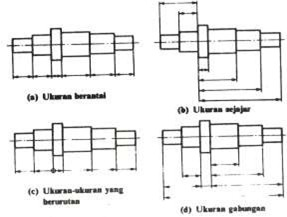
\includegraphics[width=.85\textwidth]{../figures/pemberian_ukuran.jpg}}

\end{frame}


\begin{frame}[mytitle=standard,t,mycolor=digiPH_ubcblue,dark]\frametitle{Aturan Penempatan Angka Ukuran}

	\begin{center}
		Penempatan angka ukuran pada gambar teknik:
	\end{center}

	\begin{itemize}
		\item Ditulis 1 mm di atas garis ukur
		\item Diletakkan di tengah garis ukur
		\item Harus mudah dibaca secara horizontal dan vertikal
		\item Angka ukuran harus jelas dan teratur
	\end{itemize}
\end{frame}

\begin{frame}[mytitle=center,t,mycolor=digiPH_red,dark]\frametitle{Satuan pada Gambar Teknik}

	Pada gambar teknik:

	\begin{itemize}
		\item Satuan yang digunakan adalah milimeter (mm)
		\item Satuan tidak perlu dituliskan
	\end{itemize}

	Contoh:

	\txt{digiPH_ocean}{digiPH_white}{50 (berarti 50 mm)}

	Jika menggunakan satuan lain:
	Satuan harus dicantumkan

	\txt{digiPH_ocean}{digiPH_blue}{Contoh:
		2 in (inchi)}
\end{frame}


\begin{frame}[mytitle=standard,t,mycolor=digiPH_gray,light]
	\includegraphics<1>[width=.82\textwidth]{../figures/tandapanah.png}
	\includegraphics<2>[width=.82\textwidth]{../figures/angka_bentuk_miring.jpg}
	\includegraphics<3>[width=.82\textwidth]{../figures/ukuran_bantu.png}
	\includegraphics<4>[height=.85\textheight]{../figures/ukuranluardalam.jpg}
\end{frame}

\begin{frame}[mytitle=center,t,mycolor=digiPH_white,light]\frametitle{Tugas Kelas}

	\begin{center}
		Buat \Huge Ukuran \normalsize Gambar
	\end{center}
\end{frame}















\end{document}
